\part{Suites récurrentes}

\begin{defn}
	On dit que $u$ est une suite récurrente linéaire d'ordre 2 à coefficients constants s'il existe $(a,b)\in \C$ tels que \[
		\forall n \in \N, u_{n+2} = au_{n+1} + bu_n
	\]
	L'équation caractéristique associée est \[
		(C): z^2 = az + b \text{ avec } z \in \C
	\] 
\end{defn}

\begin{prop}
	Avec les notations précédentes,
	\begin{enumerate}
		\item Si $(C)$ a 2 racines simples $r_1\neq r_2$ alors \[
			\exists (A,B)\in \C^2, \forall n\in \N, u_n = A{r_1}^n+B{r_2}^n
			\] 
		\item Si $(C)$ a une racine double $r \in \C$ alors \[
		\exists (A,B)\in \C^2, \forall n \in \N, u_n = (An+B)r^n
		\] 
	\end{enumerate}
\end{prop}

\begin{prv}
	[Récurrence double]
\end{prv}

\begin{prop}
	avec les notations précédentes et avec $(a,b)\in \R^2$ et $(u_n)\in \R^\N$\\
	\begin{enumerate}
		\item Si $(C)$ a deux racines simples $r_1 \neq r_2$ alors \[
				\exists (A,B)\in \R^2, \forall n\in \N, u_n = A{r_1}^n + B{r_2}^n
			\]
		\item Si $(C)$ a une racine simple $r \in \R$ alors \[
			\exists (A,B) \in \R^2, \forall n \in \N, u_n = (An+B)r^n
			\]
		\item Si $(C)$ a deux racines complexes conjuguées $re^{i\theta}$ avec $r \in \R^+_* \text{ et } \theta\in \left[0, \frac{\pi}{2} \right[$ alors \[
		\exists (A,B) \in \R^2, \forall n\in \N, u_n = r^n(A\cos(n\theta) + B \sin(n\theta))
		\] \qed
	\end{enumerate}
\end{prop}

\begin{rmk}
	\'Etude de $u_{n+1} = f(u_n)$
	\begin{enumerate}
		\item On choisit rapidement la fonction $f$ (au moins le tableau de variation)
		\item[1'.] ({\sc optionnel}) on représente graphiquement la fonction $f$ et la droite d'équation $y=x$ pour conjecturer sa limite
		\item On utilise le tableau de variation pour vérifier que $(u_n)$ est bien définie par récurrence \[
			P(n):\text{"$u_n$ existe et $u_n \in \mathcal{D}_f$"}
			\]
		\item On étudie le signe de $f(x)-x$
		\item On cherche les intervalles stables par  $f$: \[
				f(I)\subset I
			\] les plus petits possible (ça permet de montrer que la suite est majorée (minorée) en particulier ceux sur lesquels $f(x)-x$ ne change pas de signe
		\item[4'.] Donc on utilise le théorème de la limite monotone
		\item[4''.] Sinon, on essaie l'inégalité (voir théorème) des accroissements finis: \\
			Soit $\ell$ un point fixe de $f$: $f(\ell) = \ell$ \[
			\forall n\in \N, \left| u_{n+1} - \ell \right| =  \left| f(u_n) - f(\ell) \right| = M\left| u_n-\ell \right|
			\] où M est un majorant de $\left| f \right|$ \\
			Si $0\le M\le 1$ alors \[
			\forall n\in \N, \left| u_n-\ell \right| \le M^n\left| u_n-\ell \right| \tendsto{n\to +\infty} 0
			\] donc $u_n\tendsto{n \to +\infty} \ell$
		\item si $(u_n)$ a une limite et si $f$ continue alors $\lim(u_n)$ est une point fixe de $f$
	\end{enumerate}
\end{rmk}

\begin{exm}
	\begin{enumerate}
		\item \[
		\begin{cases}
			u_{n+1} = \cos(u_n)\\
			u_0\in \left] 0,1 \right[
		\end{cases}
		\]
		\begin{center}
			\begin{tikzpicture}
				\tkzTabInit[nocadre]{$x$/1,$f$/2}{$0$, $1$, $\frac{\pi}{2}$}
				\tkzTabVar{+/$1$,R,-/$0$}
			\end{tikzpicture}
		\end{center}
		On pose $g: x \mapsto \cos(x)-x$ dérivable et \\$\forall x\in  \left[ 0,1 \right], g'(x)=-\sin(x)-1 \le 0$ 
		
		\begin{center}
			\begin{tikzpicture}
				\tkzTabInit[nocadre]{$x$/1,$g$ /2}{$0$, $1$}
				\tkzTabVar{+/$1$,-/$g(1)<0$}
				\tkzTabVal12{0.5}{$\alpha$}0
			\end{tikzpicture}
		\end{center}
		\begin{center}
			\begin{tikzpicture}
				\tkzTabInit[nocadre]{$x$/1,$f$ /2,$f(x)-x$/1}{$0$, $\alpha$,$1$}
				\tkzTabVar{+/$1$,R,-/}
				\tkzTabVal13{0.5}{$\alpha$}0
				\tkzTabLine{,+,z,-,}
			\end{tikzpicture}
		\end{center}
		\begin{align*}
			\forall x\in \left[ 0,1 \right], \left| f'(x) \right| &= \left| -\sin(x) \right|  \\
			&= \sin(x) \le \sin(1) < 1 \\
		\end{align*}\[
		\forall n, \left| u_{n+1}-\alpha \right| = \left| f(u_n) - f(\alpha) \right|  \le \sin(1)\left| u_n-\alpha \right| 
		\] donc \[
		\forall n, \left| u_n-\alpha \right| \le \underbrace{\sin^n(1)}_{\tendsto{n\to +\infty}0} \left| u_0-\alpha \right| 
		\] Donc, $u_n\tendsto{n\to +\infty}\alpha$
	\end{enumerate}
\end{exm}
